\begin{center}
\textbf{COMO INSTALAR EL GESTOR DE BASE DE DATOS DE ORACLE EN WINDOWS SERVER 2012}
\end{center}

\begin{flushleft}
Instalar setup.exe del Sistema Gestion de Base de Datos Oracle 11g\\
Ejecutar instalador de SGBD Oracle 11g y aceptar instalación
\begin{center}
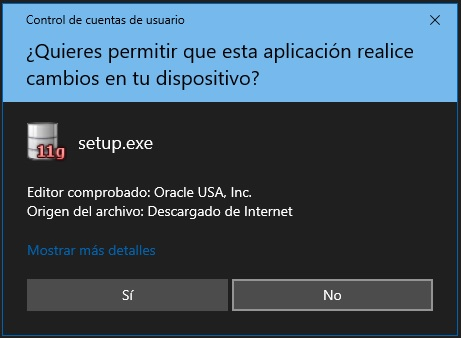
\includegraphics{images/image-01}\\
\end{center}
Nos aparecerá esta ventana en la cual esperaremos a que cargue la parte gráfica del instalador\\
\begin{center}
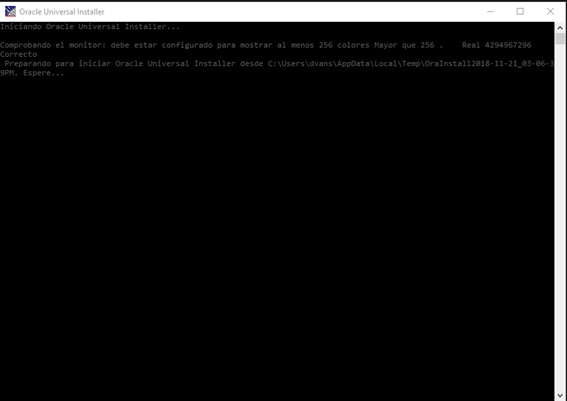
\includegraphics{images/image-02}\\

\includegraphics{images/image-03}\\
\end{center}
Nos saldrá una ventana en donde colocamos que si deseamos continua\\
\begin{center}
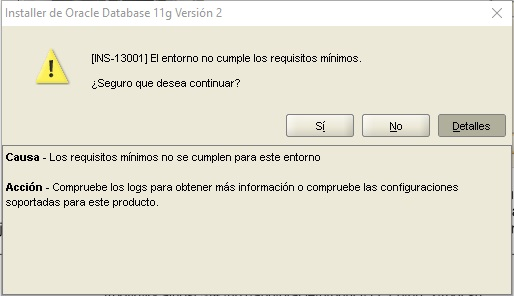
\includegraphics{images/image-04}\\
\end{center}
En esta parte presionamos en el boton siguiente\\
\begin{center}
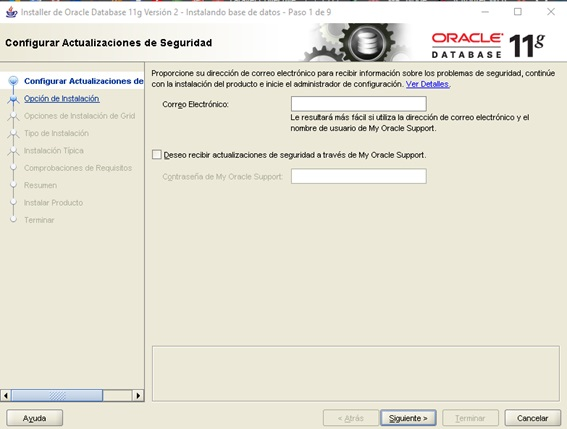
\includegraphics{images/image-05}\\
\end{center}
Nos saldrá esta ventana en el cual presionamos en el botón no porque no asignamos un correo\\
\begin{center}
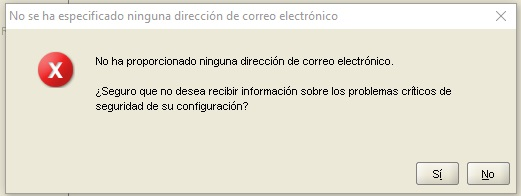
\includegraphics{images/image-06}\\
\end{center}
Selecionamos la opcion Crear y configurar base de datos , luego presionamos el boton siguiente\\
\begin{center}
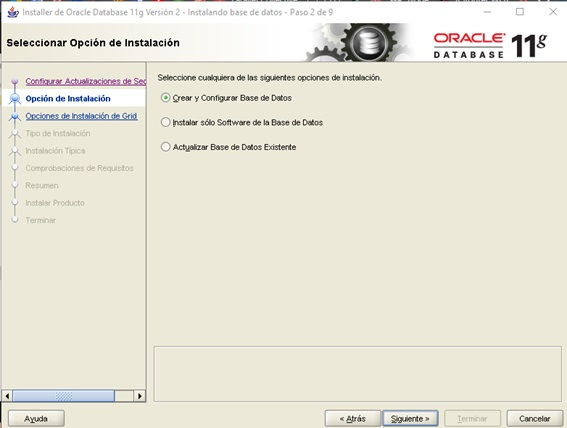
\includegraphics{images/image-07}\\
\end{center}
\end{flushleft}